\subsection{Location}
% metatext
In order to be able to locate a user and to construct routes, it is necessary to collect location data. 
The location data should only be collected under certain circumstances, such as when the user is driving in a vehicle. 
Such collection of location data can be done by using already existing services, such as the Google Play Service.

% something
Location data in RideShare is only useful if it is formatted in GPS coordinates, stored in a collection that represents a route from A to B.
There are several ways to collect location data. 
One of them is by developing a component to do so on the android device. 
Another way is to use already existing services, such as one of the Google Play Services.
%We have decided to use Google Play Services as they are well tested, and provide a reliable foundation.

To use Google Play Services, a client library much be included in the app, which will communicate via inter-process communication to the Google Play Services which is already existing on every android device. 
When the application is connected to the Google Play Services, it will automatically receive silent updates regularly, to acquire new features and bug fixes to the used services. 
This is illustrated in Figure \ref{fig:gapifigure}\cite{GapiOverview}.

\begin{figure}[h]
	\centering
	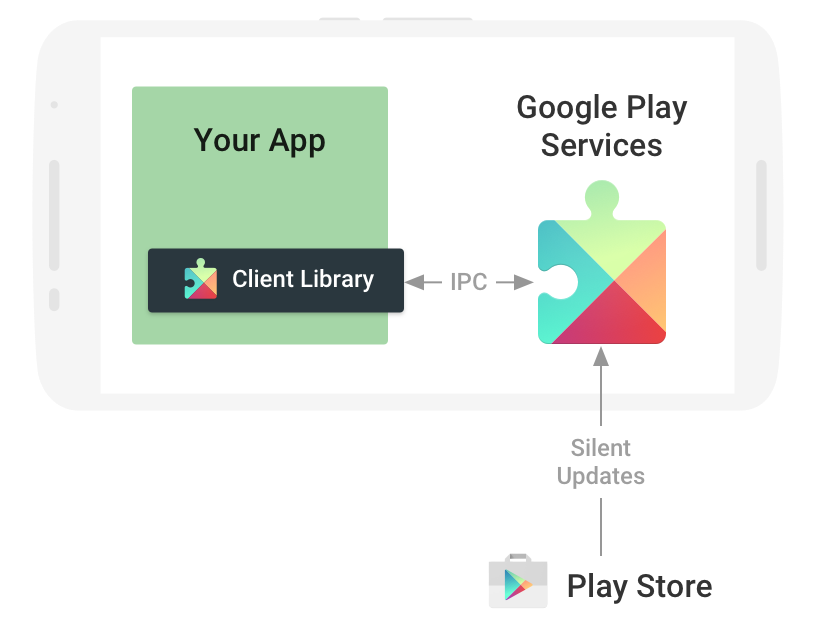
\includegraphics[width=0.7\textwidth]{figures/play-services-diagram.png}
	\caption{Google Play Services communication\cite{GapiFigure}}
	\label{fig:gapifigure}
\end{figure}

\todo{Skal måske flyttes}
The Google Play Services are restricted, and are not supporting devices with Android versions lower than 2.3. 
This limits the backwards compatibility, but the app is already restricted to Android 5 and newer, and has no influence on the target audience.
%This means that the application will not be backwards compatible as we have chosen only to focus on devices of Andorid version 2.3 and newer.

The Google Play Services will allow the application to collect location data, but it is not doing so solely using the GPS in the device. 
The location service utilizes both network location and GPS to estimate a position as precise as possible \cite{GapiLocation}. 
To ensure the collected location data is relevant, it is needed to store data only when the user is traveling by vehicle.
The Google Play Services provides a service to determine the user's activity, called Activity recognition. 

Activity recognition is a service that uses several sensors on the device to determine what kind of activity the user is currently performing, therein driving, walking, etc.
The service will return a probability level from 1 to 100, where 100 is certain that a user is performing the activity.
The activity recognition will be used to ensure unnecessary data will be stored on the database. 
It may prevent some dirty data to be stored, that could be mistaken as routes from one location to another, which were not to be considered in this application in the first place.\todo{hard to understand} 
When a user is in a vehicle with a probability level above 75 \%\todo{placeholder}, data should be stored and used for computations.

The application must be running in the background while the device is turned on, for it to be able to differ between the users activity at all times and collect data. 
It is chosen only to collect location data from the GPS every two minutes\todo{placeholder}, while in a vehicle, to reduce load\todo{what load?} and improve battery life. 
Every location collected during the driving activity must be appended to a list that represents an entire route when the driving activity ends.

When the activity change from vehicle to any other activity, the application will send the list of locations to the RideShare server, where it will take over the processing. 